\documentclass[
	fontsize=11pt,
	paper=a4,
	foldmarks=false
]{scrartcl}

\input{../manuscript/preamble}
\usepackage{response}


\setkomavar{signature}{Yang Zhao, Hongyu Li, Bruno Clerckx, and Massimo Franceschetti}
\setkomavar{date}{\today}
\setkomavar{subject}{Response to Decision on Manuscript T-SP-33360-2025}

\begin{document}
\begin{letter}{%
		Prof. Wei Yi\\
		Associate Editor\\
		IEEE Transactions on Signal Processing
	}
	\opening{Dear Editor and Reviewers,}
	Thank you for giving us an opportunity to revise the paper ``MIMO Channel Shaping and Rate Maximization Using Beyond-Diagonal RIS''.
	Your feedback and suggestions have been invaluable in helping us improve the quality of the manuscript.
	Below we prepare a point-to-point response and highlight the corresponding changes in text, where labels have been matched to the submission for your convenience.
	We hope the revisions and clarifications make the manuscript meet the TSP publication standards.
	\closing{Yours sincerely,}
\end{letter}


\begin{editor}
	\summary{
		The paper has been improved after this round of revision. However, reviewers still pointed out several critical issues regarding the novelty, practical merit, performance assessment of the paper. For example, one reviewer criticized that the rate maximization problem is actually extensively studied in existing papers and solved by different methods, by different algorithms, e.g., \cite{Zhou2023}. The application of the derived bounds on \glspl{sv} on \gls{bd}-\gls{ris} channel has been well established in early papers, e.g., \cite{Rong2009a}. I am deciding on the major revision decision. However, in the revised version, the authors need to clarify the above-mentioned very fundamental issues, otherwise the paper can still be rejected.
	}

	\reply{
		We appreciate your feedback and summary again.

		In \cite{Zhou2023}, the authors considered an energy efficiency maximization problem for \emph{multi-user \gls{miso}} downlink systems.
		A \gls{pdd} method was proposed for symmetric \gls{bd}-\gls{ris} design, which is a two-layer procedure alternating between the primal variables in the inner layer and the penalty coefficient in the outer layer.
		% While it {might} be extended to solving problem \eqref{op:rate},
		The \gls{pdd} method is often used to tackle coupled constraints (e.g., \gls{sinr} threshold involving both transmit/receive beamforming and BD-RIS matrices) and is notoriously tricky to implement.
		Invoking \gls{pdd} for \gls{mimo} rate maximization problem \eqref{op:rate_ris} is theoretically feasible but computationally very inefficient.
		% For example, to provide a stationary solution, it takes $\mathcal{O}(N_{\mathrm{s}}^2)$
		% to provide a stationary solution for diagonal and fully-connected \gls{bd}-\gls{ris}
		% For example, \gls{pdd} incurs $\mathcal{O}(N_{\mathrm{s}}^2)$ and $\mathcal{O}(N_{\mathrm{s}}^4)$ respectively to provide a stationary solution for \gls{d}-\gls{ris} and fully-connected \gls{bd}-\gls{ris} \cite[Table I]{Zhou2023}, while our proposed geodesic \gls{rcg} Algorithm \ref{ag:rcg} only takes $\mathcal{O}(N_{\mathrm{s}})$ and $\mathcal{O}(N_{\mathrm{s}}^3)$ respectively.
		For example, \gls{pdd} requires $\mathcal{O}(N_{\mathrm{s}}^2)$ and $\mathcal{O}(N_{\mathrm{s}}^4)$ flops to obtain a stationary solution for \gls{d}-\gls{ris} and fully-connected \gls{bd}-\gls{ris}, respectively \cite[Table I]{Zhou2023}, whereas our proposed geodesic \gls{rcg} Algorithm~\ref{ag:rcg} achieves the same performance with respectively $\mathcal{O}(N_{\mathrm{s}})$ and $\mathcal{O}(N_{\mathrm{s}}^3)$ flops.
		The latter exploits the structure of the block-unitary constraint for acceleration and can accommodate for the symmetric constraint when necessary (as discussed in Section \ref{sc:ris_symmetry}).

		\change{
			When it comes to signal processing, existing works have mainly invoked the {quasi-Newton} method \cite{Shen2020a}, the \gls{pdd} method \cite{Zhou2023}, and the generic (i.e., non-geodesic) \gls{rcg} method \cite{Li2023c} for the optimization of \gls{bd}-\gls{ris}.
			The first solves an unconstrained problem and projects the solution back to the feasible domain without optimality guarantee.
			The second alternates between the primal variables in the inner layer and the penalty coefficient in the outer layer.
			It is often used to tackle coupled constraints (e.g., \gls{sinr} thresholds under active and passive beamforming) and can be computationally expensive (e.g., $\mathcal{O}(N_{\mathrm{s}}^2)$ for \gls{d}-\gls{ris} and $\mathcal{O}(N_{\mathrm{s}}^4)$ for fully-connected \gls{bd}-\gls{ris}) \cite[Table I]{Zhou2023}.
			The third applies the conjugate gradient method on generic Riemannian manifolds.
			Each iteration consists of an addition on the tangent space and a retraction to the feasible domain, which constitutes a zigzag path departing from and returning to the manifold.
			However, none of them effectively exploits the special structure of \gls{bd}-\gls{ris} for accelerated convergence.
		}

		We would also like to point out that \cite{Rong2009a}, mentioned by the editor, actually investigated the optimal beamforming design for multi-hop \emph{\gls{af} relays} with \emph{no channel \gls{sv} manipulation bounds} taken into account.
		Those are active devices that consume power to amplify the signal with noise.
		The optimal structure of \gls{af} relays \cite[(17)]{Rong2009a} comes in the form
		\begin{equation}
			\mathbf{F} = \mathbf{V}_{\mathrm{B}} \mathbf{\Lambda} \mathbf{U}_{\mathrm{F}}^\mathsf{H},
		\end{equation}
		where $\mathbf{\Lambda}$ is a diagonal matrix that models the effect of relay power allocation.
		The aim of \cite{Rong2009a} is to show, as quoted from the authors, ``The optimal source and relay matrices jointly diagonalize the multi-hop \gls{mimo} relay system into a set of parallel scalar channels.''
		On the other hand, our paper aims to characterize the fundamental limits of \gls{bd}-\gls{ris} in \gls{mimo} channel \glspl{sv} shaping.
		\gls{bd}-\gls{ris} can only manipulate the phase and amplitude of the signal by passive scattering without amplification, which is fundamentally different from \gls{af} relays in terms of hardware architecture, power consumption, and noise characteristics.
		It just happens that \emph{the mathematical modeling of \gls{af} relays of unit power coincide with the modeling of fully-connected \gls{bd}-\gls{ris},} and thus the rate-optimal solutions.
		The underlying physical constraints and the resulting practical implications are clearly distinct.

		\change{
			For example, the rate maximization problem \cite{Bartoli2023} has only been tacked in the special case where the direct channel is negligible and the \gls{bd}-\gls{ris} is fully-connected.
			Under those conditions, the mathematical modeling of \gls{bd}-\gls{ris} coincides with that of \gls{af} relay of unit power, although the operation mechanism and noise characteristics are clearly distinct.
		}

		\change{
			We notice that \eqref{eq:ris_nd_power_max} and \eqref{eq:ris_nd_power_min} are special cases of \eqref{eq:ris_nd_sv_indl_max} and \eqref{eq:ris_nd_sv_indl_min} with $\mathbf{P} = \mathbf{I}$ and $\mathbf{Q} = \mathbf{J}$, which also attain the right and left halves of \eqref{iq:sv_nd_extreme}, respectively.
			That is to say, there exists a closed-form \gls{bd}-\gls{ris} solution \eqref{eq:ris_nd_power_max} maximizing the channel power gain that is also optimal for wireless power transfer.
			We will shortly see that this solution also achieves the channel capacity.
			The upper bound \eqref{eq:ris_nd_power_max} is also reminiscent of the optimal \gls{af} relay beamforming design \cite[(16), (17)]{Rong2009a} where the diagonal power allocation matrices boil down to $\mathbf{I}$ due to the passive nature of \gls{ris}.
		}

		We also supplied extensive theoretical studies of \gls{bd}-\gls{ris} in Propositions \ref{pp:dof} -- \ref{pp:nd} and the resulting Corollaries, most of which are new results to the topic.
		The comments from the reviewers have also been addressed to our best efforts as reflected below.
		Therefore, we would like to politely invite the editor to reconsider the decision for this manuscript.
	}

\end{editor}

\begin{reviewer}
	\summary{
		The authors have addressed my concerns.
	}

	\reply{
		Thank you for your positive feedback and continued support.
	}
\end{reviewer}


\begin{reviewer}
	\summary{
		This paper explores potentials of a new type of \gls{ris}, specifically adopting a \gls{bd} scattering model, in shaping point-to-point \gls{mimo} channels for improved wireless performance. The authors derive analytical bounds under specific scenarios and propose a numerical optimization method for broader shaping problems, both of which are verified by simulation results. The paper tackles an important and timely question regarding the channel shaping capabilities of passive \gls{ris}, particularly moving beyond the conventional \gls{d}-\gls{ris} model. The singular value analysis and optimization is a fresh and relevant perspective in the field. However, there are areas which need further improvement:
	}

	\comment{
	Implementation of \gls{bd}-\gls{ris}: The paper could benefit from more thorough discussions on practical implementation challenges of \gls{bd}-\gls{ris}, including manufacturing complexity, calibration, and hardware imperfections. Addressing these would enhance the paper's practical relevance and applicability.
	}

	\reply{
		Thank you very much for the suggestion. The practical implementation of \gls{bd}-\gls{ris} is a profound and challenging issue that deserves further discussion. Some of the authors have a newly released preprint \cite{Li25x} that covers the topic in great depth. It has been discussed lightly in this submission due to the page limitation, and we appreciate your understanding on this point.
	}

	\change{
		The main manufacturing complexity of \gls{bd}-\gls{ris} lies in the design and implementation of the circuit network.
		Fortunately, novel topologies such as tree- and forest-connections have been proposed to reduce the number of components for a flexible cost-performance tradeoff \cite{Nerini2024}.
		Other practical challenges such as channel estimation \cite{Li2024}, mutual coupling \cite{Li2023f}, wideband modelling \cite{Li2024a}, multi-sector coverage \cite{Li2023c}, and hardware implementation \cite{Tapie25e} have also been studied in recent literature.
		\gls{bd}-\gls{ris} has been proved to achieve higher spectral efficiency than \gls{d}-\gls{ris} and higher energy efficiency than active \gls{ris} and \gls{af} relay \cite{Santamaria2023,Fang2023,Zhou2023}.
	}

	\comment{
	Comparison between \gls{rcg} methods: The link could be highlighted by mentioning that the non-geodesic update (additive + retraction) effectively employs a first-order Taylor approximation of the geodesic update (multiplicative via matrix exponential), thus necessitating the retraction step to ensure iterates remain on the manifold.
	}

	\reply{
		This is indeed a great point to highlight as it can help the readers to understand the connection and difference between the two \gls{rcg} methods.
		We have updated the context as follows.

		\change{
			Algorithm~\ref{ag:rcg} summarizes the proposed geodesic \gls{rcg} method with sequential group-wise updates.
			Each iteration leverages Lie algebra to perform a multiplicative update \eqref{eq:geodesic_tran} along the geodesics of the Stiefel manifold.
			This appropriate parameter space leads to faster convergence and easier step size tuning.
			We remark that the additive update of the non-geodesic \gls{rcg} can be interpreted a first-order Taylor approximation to the multiplicative update of the proposed geodesic \gls{rcg}, thus necessitating a retraction step to remain on the manifold.
			% Compared to the non-geodesic approach, it leverages Lie algebra to replace the add-then-retract update with a multiplicative update \eqref{eq:geodesic_tran} along the geodesics of the Stiefel manifold.
			% This appropriate parameter space leads to faster convergence and easier step size tuning.
			% In fact, the non-geodesic approach
			% Convergence to a local optimum is guaranteed if not initialized at a stationary point.
			The group-wise updates can be performed in parallel to facilitate large-scale \gls{bd}-\gls{ris} design problems.
			One may also operate on $\mathbf{\Theta}$ and pinching (i.e., keeping the main block diagonal and nulling the rest) \eqref{eq:gradient_eucl} to unify the step size selection for further acceleration.
		}
	}

	\comment{
	Applicability to other \gls{bd}-\gls{ris} models: The focus is strongly on the group-connected \gls{bd}-\gls{ris} versus \gls{d}-\gls{ris}. The authors could clarify how the proposed methods and results might extend to other \gls{bd}-\gls{ris} models, such as multi-sector or multi-layer configurations. This would broaden the applicability of the findings and provide a more comprehensive understanding of the \gls{ris} landscape.
	}

	\reply{
		We appreciate the reviewer for mentioning this point.
		While the analysis and optimization methods in this paper have been tailored for the group-connected \gls{bd}-\gls{ris} in shaping point-to-point \gls{mimo} channels, we believe they can offer an initial benchmark for other models.
		We have added a paragraph in the conclusion to clarify this point.

		\change{
			The analysis and optimization methods in this paper have been tailored for group-connected \gls{bd}-\gls{ris}.
			Extension to other architectures remains a promising direction for future research.
			We believe that one straightforward extension to the multi-sector model \cite{Li2023c} is to retrieve the optimal scattering matrix for each sector individually by our method and then play with the power splitting factors.
			Meanwhile, transitioning towards multi-layer \gls{ris} models \cite{An23b} mirrors that from single-hop to multi-hop \gls{af} relays; interested readers may be inspired by \cite{Rong2009a} on this point.
		}
	}

	\comment{
	Readability of the Technical Parts: The readability of the paper could be improved by having more intuitions and/or explanations after important theorems/lemmas/corollaries.
	}

	\reply{
		Apart from Examples \ref{eg:dof} and \ref{eg:shaping_bounds}, we have now added explanations and typical use cases after those theoretical results to help the readers understanding their meanings and applications.
		The logic flow and wordings have also been carefully reworked.
		Please refer to Response \ref{re:3.1} and the manuscript for details.
	}
\end{reviewer}


\begin{reviewer}
	\summary{
		The reviewer appreciates the authors’ efforts to prepare the revision. The reviewer has the following concerns:
	}

	\comment{
	The authors provide a bunch of bounds (Prop. \ref{pp:rd}) on \glspl{sv} of \gls{bd}-\gls{ris} channels. The significance of these bounds is unclear. What can these bounds be used for? One possible solution lies in the achievable maximal channel capacity (Corollary \ref{co:nd_capacity_snr_general}). However, this result (the well-known forward and backward channel alignment) has long been established, e.g., \cite{Rong2009a}. Especially, the bounds developed in corollaries \ref{co:nd_sv_prod_subset}-\ref{co:nd_sv_indl} are a great number of inequalities coupling with each other. How could these bounds be used?
	}

	\reply{
		\label{re:3.1}
		We appreciate the reviewer for the clinical questions and aim to answer them one-by-one below.
		\begin{itemize}
			% \item Proposition \ref{pp:rd} shows that
			\item The \gls{sv} bounds in Proposition \ref{pp:rd} complements the \gls{dof} result in Proposition \ref{pp:dof} by quantifying the dynamic range of extreme singular values in low-multipath scenarios. They reveal a saturation effect of increasing the number of \gls{bd}-\gls{ris} elements and group size in enhancing channel shaping capability. Therefore, the bounds can be used to guide practical \gls{ris} configurations, especially in millimeter-wave and terahertz systems under sparse environment, for a balanced performance gain and hardware complexity.
			Another use case is strategic network planning where the bounds can help compare the shaping capabilities of a single massive \gls{ris} versus multiple smaller distributed ones without actually developing them.
			\change{
				We emphasize that Proposition \ref{pp:rd} and Corollary \ref{co:los} apply to both \gls{d}- and \gls{bd}-\gls{ris} configurations regardless of the status of the direct channel.
				Out of $2N$ bounds in \eqref{iq:sv_rd} or \eqref{iq:sv_los}, $N$ of them can be \emph{simultaneously} tight as $N_\mathrm{S} \to \infty$, namely when the direct channel becomes negligible.
				For a finite $N_\mathrm{S}$, the \gls{ris} may prioritize a subset of those by aligning the corresponding modes.
				We will show by simulation that \gls{bd}-\gls{ris} outperforms \gls{d}-\gls{ris} on this purpose.
				Proposition \ref{pp:rd} complements the \gls{dof} result in Proposition \ref{pp:dof} by quantifying the dynamic range of extreme singular values in low-multipath scenarios.
				They reveal a diminishing return of increasing the number of \gls{bd}-\gls{ris} elements and group size in enhancing channel shaping capability. Therefore, the bounds can be used to guide practical \gls{ris} configurations, especially in millimeter-wave and terahertz systems under sparse propagation environment, for a balanced performance-complexity tradeoff.
				Next, we progress to quantify the limits of singular value redistribution when the direct channel is negligible.
			}
			\item The bounds in Corollary \ref{co:nd_sv_prod_subset} sketch the outer bounds of the entire achievable channel \gls{sv} region under the assumption of negligible direct channel and fully-connected \gls{bd}-\gls{ris}. While direct application of every inequality within is not straightforward, they indeed provide a rich theoretical foundation and ultimate performance limit for \gls{mimo} channel shaping using \gls{bd}-\gls{ris}. One may choose any subset of those bounds for specific wireless applications and metrics, and some examples are given in Corollaries \ref{co:nd_sv_prod_tail} and \ref{co:nd_sv_indl}. In the revised manuscript, we have also added simulation results comparing the outer bounds in Corollary \ref{co:nd_sv_prod_subset} and the achievable region obtained by solving the optimization problem \eqref{op:pareto} in Fig. \ref{fg:singular_region}.
			\change{
				\setcounter{figure}{1}
				\begin{figure}[H]
					\centering
					\subfloat[Top view]{
						\label{fg:singular_region_top}
						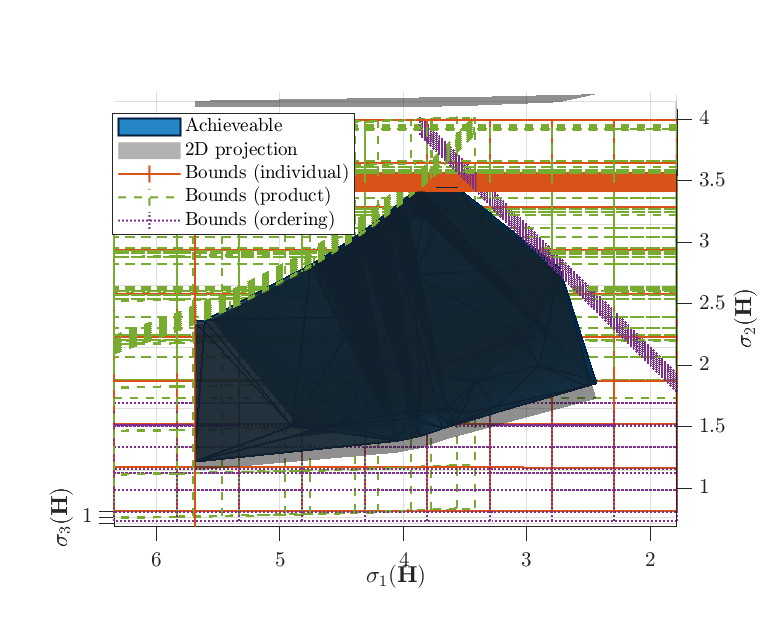
\includegraphics[width=0.485\columnwidth]{../assets/simulation/pc_singular_region_top.eps}
					}
					% \\
					% \subfloat[Front view]{
					% 	\label{fg:singular_region_front}
					% 	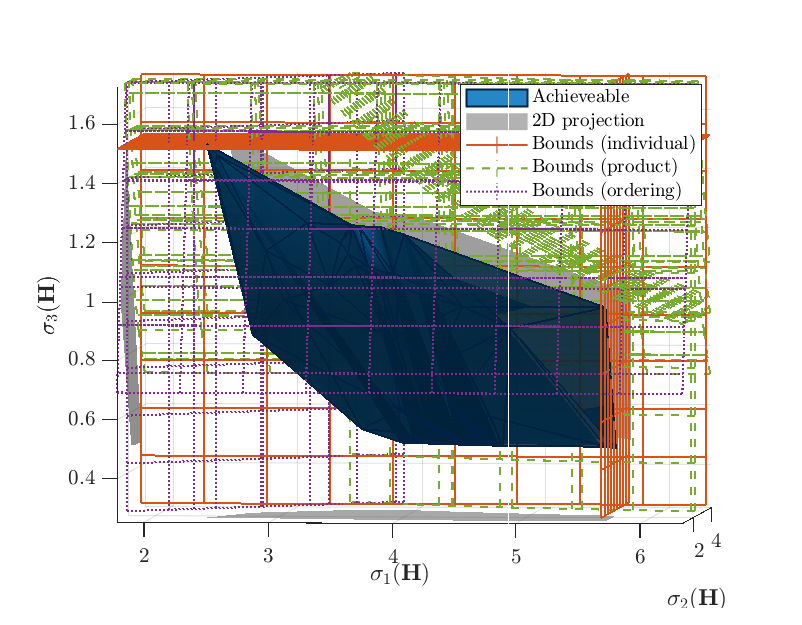
\includegraphics[width=0.485\columnwidth]{../assets/simulation/pc_singular_region_front.eps}
					% }
					\subfloat[Side view]{
						\label{fg:singular_region_side}
						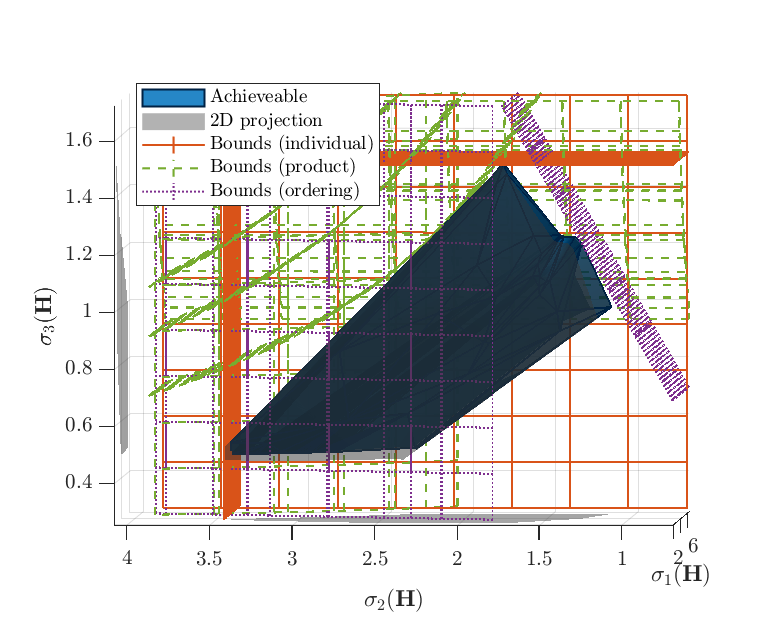
\includegraphics[width=0.485\columnwidth]{../assets/simulation/pc_singular_region_side.eps}
					}
					\caption{Theoretical singular value outer bounds \eqref{iq:horn} (uniformly-spaced mesh grids) vs achievable singular value region by solving \eqref{op:pareto} (solid dark shape) for one channel realization, where $N_\mathrm{T}=N_\mathrm{S}=N_\mathrm{R}=3$, the direct channel is negligible, and the \gls{bd}-\gls{ris} is fully-connected. Small offsets are introduced on both views such that the active bounds are highlighted by densely-spaced curves/lines that marginally overlap the region from above. The achievable region lies entirely within the intersection of the bounding surfaces in the 3D space.}
					\label{fg:singular_region}
				\end{figure}

				Fig. \ref{fg:singular_region} compares the achievable singular value region obtained by solving problem \eqref{op:pareto} and its outer bounds suggested by Corollary \ref{co:nd_sv_prod_subset}.
				Here $\bar{N}=N_\mathrm{T}=N_\mathrm{S}=N_\mathrm{R}=3$ and the bounds are enumerated as
				\begin{subequations}
					\begin{equation}
						\label{iq:sv_3_individual}
						\begin{gathered}
							\sigma_1(\mathbf{H}) \le \sigma_1(\mathbf{H}_\mathrm{B}) \sigma_1(\mathbf{H}_\mathrm{F}), \quad
							\sigma_2(\mathbf{H}) \le \sigma_1(\mathbf{H}_\mathrm{B}) \sigma_2(\mathbf{H}_\mathrm{F}), \\
							\sigma_2(\mathbf{H}) \le \sigma_2(\mathbf{H}_\mathrm{B}) \sigma_1(\mathbf{H}_\mathrm{F}), \quad
							\sigma_3(\mathbf{H}) \le \sigma_1(\mathbf{H}_\mathrm{B}) \sigma_3(\mathbf{H}_\mathrm{F}), \\
							\sigma_3(\mathbf{H}) \le \sigma_2(\mathbf{H}_\mathrm{B}) \sigma_2(\mathbf{H}_\mathrm{F}), \quad
							\sigma_3(\mathbf{H}) \le \sigma_3(\mathbf{H}_\mathrm{B}) \sigma_1(\mathbf{H}_\mathrm{F}),
						\end{gathered}
					\end{equation}
					\begin{equation}
						\label{iq:sv_3_product}
						\begin{gathered}
							\sigma_1(\mathbf{H}) \sigma_2(\mathbf{H}) \le \sigma_1(\mathbf{H}_\mathrm{B}) \sigma_2(\mathbf{H}_\mathrm{B}) \sigma_1(\mathbf{H}_\mathrm{F}) \sigma_2(\mathbf{H}_\mathrm{F}), \\
							\sigma_1(\mathbf{H}) \sigma_3(\mathbf{H}) \le \sigma_1(\mathbf{H}_\mathrm{B}) \sigma_3(\mathbf{H}_\mathrm{B}) \sigma_1(\mathbf{H}_\mathrm{F}) \sigma_2(\mathbf{H}_\mathrm{F}), \\
							\sigma_1(\mathbf{H}) \sigma_3(\mathbf{H}) \le \sigma_1(\mathbf{H}_\mathrm{B}) \sigma_2(\mathbf{H}_\mathrm{B}) \sigma_1(\mathbf{H}_\mathrm{F}) \sigma_3(\mathbf{H}_\mathrm{F}), \\
							\sigma_2(\mathbf{H}) \sigma_3(\mathbf{H}) \le \sigma_1(\mathbf{H}_\mathrm{B}) \sigma_2(\mathbf{H}_\mathrm{B}) \sigma_2(\mathbf{H}_\mathrm{F}) \sigma_3(\mathbf{H}_\mathrm{F}), \\
							\sigma_2(\mathbf{H}) \sigma_3(\mathbf{H}) \le \sigma_2(\mathbf{H}_\mathrm{B}) \sigma_3(\mathbf{H}_\mathrm{B}) \sigma_1(\mathbf{H}_\mathrm{F}) \sigma_2(\mathbf{H}_\mathrm{F}), \\
							\sigma_2(\mathbf{H}) \sigma_3(\mathbf{H}) \le \sigma_1(\mathbf{H}_\mathrm{B}) \sigma_3(\mathbf{H}_\mathrm{B}) \sigma_1(\mathbf{H}_\mathrm{F}) \sigma_3(\mathbf{H}_\mathrm{F}),
						\end{gathered}
					\end{equation}
					\begin{equation}
						\label{iq:sv_3_ordering}
						\sigma_1(\mathbf{H}) \ge \sigma_2(\mathbf{H}) \ge \sigma_3(\mathbf{H}),
					\end{equation}
				\end{subequations}
				where \eqref{iq:sv_3_individual}, \eqref{iq:sv_3_product} are explicit results of \eqref{iq:horn} while \eqref{iq:sv_3_ordering} denotes the ordering of singular values.
				Those are labeled respectively as `Bounds (individual)', `Bounds (product)', and `Bounds (ordering)' in Fig. \ref{fg:singular_region}.
				The two views confirm that the theoretical outer bounds are not everywhere tight with many entries being redundant, but they provide a conservative estimate of the achievable singular value region.
				Importantly, the vertices of the region are always on the boundary, which implies that those can be achieved in the closed form without performing optimization.
			}
			\item The bounds in Corollary \ref{co:nd_sv_prod_tail} reveal the upper (resp. lower) bound on the product of some largest (resp. smallest) channel \glspl{sv}. These bounds can be applied, for instance, as a shortcut to establish the upper bound of \gls{bd}-\gls{ris}-aided \gls{mimo} channel capacity at extreme \glspl{snr}.
			\change{
				Corollary \ref{co:nd_sv_prod_tail} reveals the shaping limits on the product of some extreme channel singular values.
				The lower bounds \eqref{iq:sv_nd_prod_smallest} coincide at zero when $\bar{N} \ne N$ (i.e., $N_\mathrm{T} = N_\mathrm{S} = N_\mathrm{R}$ being false).
				These bounds can be applied, for instance, as a shortcut to establish the capacity of \gls{bd}-\gls{ris}-aided \gls{mimo} channels at extreme \gls{snr}, as shown in Corollary \ref{co:nd_capacity_snr_extreme}.
				In the special case $k=1$, we arrive at the upper bound on the largest channel singular value $\sigma_1(\mathbf{H}) {\le} \sigma_1(\mathbf{H}_\mathrm{B}) \sigma_1(\mathbf{H}_\mathrm{F})$.
				This is particularly useful for \gls{mimo} wireless power transfer with \gls{rf} combining where the harvested power depends merely on, and is a quartic function of, the largest channel singular value \cite{Shen2021}.
				A closed-form \gls{bd}-\gls{ris} solution to attain this upper bound can be found below.
			}
			\item The bounds in Corollary \ref{co:nd_sv_indl} reveal the shaping limits of the $n$-th largest channel \gls{sv}. These bounds enable closed-form passive beamforming, and hence fixed channel and closed-form active beamforming, for spatial multiplexing with a limited number $n$ of \gls{rf} chains. Another use case is to enhance the harvested power for \gls{mimo} wireless power transfer with \gls{rf} combining by maximizing the dominant channel \gls{sv}.
			One may also improve the channel condition number for numerically stable signal processing by maximizing the smallest channel \gls{sv}.
			\change{
				Corollary \ref{co:nd_sv_indl} and Proposition \ref{pp:rd} both reveal the shaping limits of the $n$-th largest channel singular value.
				% , which may be used to simplify the \gls{mimo} precoder design with limited number $n$ of \gls{rf} chains.
				They are derived under different assumptions are not special cases of each other.
				Importantly, Corollary \ref{co:nd_sv_indl} establishes upper and lower bounds for \emph{each} channel singular value (c.f. first and last $k$ in Proposition \ref{pp:rd}) and provides general solutions for fully-connected \gls{bd}-\gls{ris} of arbitrary (c.f. sufficiently large) size to attain the equalities.
				% These bounds can be applied, for instance, to provide a closed-form passive beamforming (and thus fixed channel and closed-form active beamforming) for spatial multiplexing with a limited number $n$ of \gls{rf} chains.
				These bounds enable closed-form passive beamforming, and hence fixed channel and closed-form active beamforming, for spatial multiplexing with a limited number $n$ of \gls{rf} chains.
				% Another use case is to enhance the harvested power for \gls{mimo} wireless power transfer with \gls{rf} combining by maximizing the dominant channel singular value \cite{Shen2021}.
				% One may also improve the channel condition number for numerically stable signal processing by maximizing the smallest channel singular value.
				We emphasize that in \eqref{eq:ris_nd_sv_indl} the mode alignment is realized by $\mathbf{V}_\mathrm{B}$ and $\mathbf{U}_\mathrm{F}$ while the ordering is enabled by permutation matrices $\mathbf{P}$ and $\mathbf{Q}$, which are special cases of $\mathbf{X}$ defined in \eqref{eq:ris_decompose_group}.
			}
			\item While \cite{Rong2009a} discussed the optimal beamforming structure for multi-hop \gls{af} relays, its focuses of channel diagonalization and relay power allocation are fundamentally different from this paper. The literature provides neither channel \gls{sv} bounds nor channel capacity bounds. Please refer to our response to the editor on this point.
		\end{itemize}
	}

	\comment{
	Prop. \ref{pp:shaping} imposes the assumption that $f(\cdot)$ must be symmetric gauge function in \glspl{sv} of $\mathbf{H}$. Note gauge function is strong assumption since it should be homogeneous and convex (e.g., \cite[Sec 3-I]{Marshall2010}) in \glspl{sv} of $\mathbf{H}$, which indeed severely restricts the range of its application. When $f(\cdot)$ is nonconvex, subdifferential ($\mathbf{D}$ in eq. \eqref{eq:shaping_subdiff}) generally does not exist. In fact, any commonly adopted performance metrics, e.g., spectral efficiency, energy efficiency, receiving power are not gauge functions (they are inhomogeneous and nonconvex).
	On the other hand, to obtain partial differential with respect to (w.r.t.) \gls{ris}, (i.e., the aim of Prop. \ref{pp:shaping}), the assumption of gauge function is unnecessary. Directly taking the derivative of $f(\cdot)$ w.r.t. \gls{ris} is more preferable.
	}

	\reply{
		We fully agree with the reviewer that enforcing $f(\mathrm{sv}(\mathbf{H}))$ as a gauge function is too restrictive and unnecessary for the shaping problem.
		In the revised manuscript, Prop \ref{pp:shaping} has been extended to locally Lipschitz functions of channel singular values.
		We sincerely appreciate your insights on this issue.

		\change{
			Below we propose a numerical method to optimize \gls{bd}-\gls{ris} for a broad class of singular value functions.
			\setcounter{definition}{2}
			\begin{definition}[Locally Lipschitz]
				A function $f: \mathbb{R}^N \to \mathbb{R}$ is locally Lipschitz if for any compact set $\mathcal{S} \subset \mathbb{R}^N$, there exists a constant $L > 0$ such that $\lvert f(\mathbf{x}) - f(\mathbf{y}) \rvert \le L \lVert \mathbf{x} - \mathbf{y} \rVert$ for all $\mathbf{x}, \mathbf{y} \in \mathcal{S}$.
			\end{definition}

			\setcounter{proposition}{3}
			\begin{proposition}
				\label{pp:shaping}
				Consider channel shaping problems of the form
				\begin{maxi!}
					{\scriptstyle{\mathbf{\Theta}}}{f\bigl(\sv(\mathbf{H})\bigr)}{\label{op:shaping}}{\label{ob:shaping}}
					\addConstraint{\mathbf{\Theta}_g^\mathsf{H} \mathbf{\Theta}_g=\mathbf{I},}{\quad \forall g,}{\label{cn:shaping_unitary}}
				\end{maxi!}
				where $f: \mathbb{R}^{N} \to \mathbb{R}$ is arbitrary locally Lipschitz function of channel singular values.
				The Clarke subdifferential of \eqref{ob:shaping} with respect to \gls{bd}-\gls{ris} block $g$ is
				\begin{equation}
					\label{eq:shaping_subdiff}
					\partial_{\mathbf{\Theta}_g^*} f\bigl(\sv(\mathbf{H})\bigr) = \conv \bigl\{ \mathbf{H}_{\mathrm{B},g}^\mathsf{H} \mathbf{U} \mathbf{D} \mathbf{V}^\mathsf{H} \mathbf{H}_{\mathrm{F},g}^\mathsf{H} \bigr\},
					% \partial_{\mathbf{\Theta}_g^*} f\bigl(\sv(\mathbf{H})\bigr) = \conv \bigl\{ \mathbf{H}_{\mathrm{B},g}^\mathsf{H} \mathbf{U} \mathbf{D} \mathbf{V}^\mathsf{H} \mathbf{H}_{\mathrm{F},g}^\mathsf{H} \bigr\},
				\end{equation}
				where $\mathbf{D} \in \mathbb{C}^{N_\mathrm{R} \times N_\mathrm{T}}$ is a rectangular diagonal matrix with $[\mathbf{D}]_{n,n} \in \partial_{\sigma_n(\mathbf{H})} f\bigl(\sv(\mathbf{H})\bigr)$, $\forall n \in [N]$, and $\mathbf{U}$, $\mathbf{V}$ are any left and right singular matrices of $\mathbf{H}$.
			\end{proposition}

			\begin{proof}
				Please refer to Appendix~\ref{ap:shaping}.
			\end{proof}

			Proposition \ref{pp:shaping} enables subgradient-based optimization for arbitrary locally Lipschitz function of channel singular values (e.g., Pareto frontier, power gain, capacity, condition number) via \eqref{eq:shaping_subdiff}.
			Next, we introduce a \emph{geodesic \gls{rcg}} method modified from \cite{Abrudan2008,Abrudan2009} for the optimization of \gls{bd}-\gls{ris}.
			Our contribution is an extension to the block-unitary case with sequential, parallel, or unified updates for accelerated convergence.
			The steps for updating $\mathbf{\Theta}_g$ at iteration $r$ are summarized below, where the gradients are replaced by Clarke subgradients for non-smooth $f$.
		}
	}

	\comment{
	The authors propose Riemannian Conjugate Gradient (\gls{rcg}) algorithm (Algorithm \ref{ag:rcg}) to optimize \gls{ris} configuration. Note CG descent on manifold is indeed well established and is widely used for optimization on manifolds, e.g., \cite{Boumal23t}. It can be implemented conveniently by off-the-shelf solvers, e.g., Manopt \cite{Boumal14a}. Then, what is the novelty or significance of Sec. \ref{sc:shaping_numerical}?
	}

	\reply{
		Manopt is indeed a canonical tool for manifold optimization. Upon inspecting the source code, we found it invokes a generic non-geodesic solver for feasible domain \texttt{stiefelcomplexfactory(n, p, k)} that does not exploit the block-unitary structure of our problem. This is also confirmed by MATLAB profiler that $~60\%$ of its running time was spent on projection (i.e. retraction from the Euclidean space to the manifold, due to non-geodesic update). This is the main bottleneck of the algorithm.
		\begin{figure}[H]
			\centering
			\includegraphics[width=0.75\columnwidth]{../assets/review/profiler.png}
			\caption{MATLAB profiler report of Manopt vs proposed \gls{rcg} on 1000 independent channel realizations. The simulation parameters are inline with Table \ref{tb:complexity_algorithm}.}
		\end{figure}


		In contrast, our proposed geodesic \gls{rcg} algorithm is tailored to group-connected \gls{bd}-\gls{ris} designs, offering significant computational advantages as discussed in context. The novelty of Section \ref{sc:shaping_numerical} lies in:
		\begin{itemize}
			\item The formulation of the channel shaping problem as an optimization problem on the product of unitary manifolds, which is a natural and appropriate setting for \gls{bd}-\gls{ris} design.
			\item The derivation of the translated Riemannian gradient at the identity of the manifold, which offers a compact expression for the geodesic update.
			\item The development of a specialized geodesic \gls{rcg} algorithm that leverages the block-unitary structure of \gls{bd}-\gls{ris} for accelerated convergence and reduced computational complexity compared to general-purpose manifold optimization solvers.
			\item The application of this algorithm to reveal the entire achievable channel \gls{sv} region, which is a novel contribution to the understanding of \gls{bd}-\gls{ris} shaping capabilities.
		\end{itemize}

		In the revised manuscript, we have added Table \ref{tb:complexity_algorithm} to benchmark the performance of two \gls{rcg} algorithms on the Pareto channel \gls{sv} problem \eqref{op:pareto}

		\change{
			\begin{table}[H]
				\caption{Performance of \gls{rcg} Algorithms on \eqref{op:pareto} with $N_\mathrm{T}=N_\mathrm{R}=4$, $L=16$}
				\label{tb:complexity_algorithm}
				\centering
				\resizebox{\columnwidth}{!}{
					\begin{tabular}{ccccccc}
						\toprule
						\multirow{2}{*}{\gls{rcg} path} & \multicolumn{2}{c}{$N_\mathrm{S}=16$} & \multicolumn{2}{c}{$N_\mathrm{S}=64$} & \multicolumn{2}{c}{$N_\mathrm{S}=256$}                                      \\
						\cmidrule(lr){2-3} \cmidrule(lr){4-5} \cmidrule(lr){6-7}
						                                & Iterations                            & Time [ms]                             & Iterations                             & Time [ms] & Iterations & Time [ms] \\
						\midrule
						Geodesic                        & 6.493                                 & 1.807                                 & 9.003                                  & 7.378     & 12.98      & 49.41     \\
						Non-geodesic (Manopt)           & 8.601                                 & 25.90                                 & 11.09                                  & 36.27     & 14.29      & 65.89     \\
						\bottomrule
					\end{tabular}
				}
			\end{table}

			Table \ref{tb:complexity_algorithm} benchmarks two \gls{rcg} algorithms on the Pareto singular value problem \eqref{op:pareto} with $N_\mathrm{T}=N_\mathrm{R}=4$ and $L=16$.
			The geodesic \gls{rcg} is implemented with pinched gradients w.r.t. $\mathbf{\Theta}$ and unified step size selection; please refer to the discussion below \eqref{eq:geodesic_tran} for details.
			The non-geodesic \gls{rcg} is implemented by \texttt{Manopt} toolbox at commit \texttt{a879a0d} \cite{Boumal14a}.
			Both algorithms employ a stopping criterion of relative change in the objective function with a tolerance of $\epsilon = \num{1e-4}$, such that the final values are identical within reasonable precision.
			The statistics are averaged over 1000 independent channel realizations.
			We observe that the non-geodesic \gls{rcg} typically requires 1 to 2 more iterations than its geodesic counterpart.
			This is because the addition is in the tangent space of the manifold and is less effective than manifold-native updates.
			When it comes to elapsed time, the geodesic \gls{rcg} is $1333\%$ faster than the non-geodesic counterpart when $N_\mathrm{S}=16$.
			The main reason is that the geodesic \gls{rcg} avoids the retraction step from the Euclidean space to the manifold.
			According to the profiler report, around $60\%$ of the non-geodesic \gls{rcg} runtime is spent on retraction, which becomes the main bottleneck of the algorithm.
			The advantage narrows down to $391.6\%$ and $33.35\%$ when $N_\mathrm{S}=64$ and $256$, respectively.
			This is because accurately evaluating matrix exponential can be time-consuming for large $N_\mathrm{S}$.
		}
	}

\end{reviewer}


\bibliographystyle{IEEEtran}
\bibliography{response}
\end{document}
